% Session 9 -- Yu-Shiba-Rusinov states: what a magnetic impurity does to a
% Placement: sec. "Impurities as diagnostics II", after equation (9.10).
% Rendered by figures/blender/s09f03_ysr.py, labels in figures/overlays/s09f03_ysr.tex.
\begin{aqmfigure}{fig:s09:ysr}{A magnetic impurity in an s-wave superconductor. (a) The
single-particle density of states. The BCS continuum, with a gap $\Delta$ and coherence peaks at the
gap edges, is almost unchanged by a \emph{non-magnetic} impurity. Such an impurity does not
distinguish up from down, so it cannot lower the energy needed to break any specific Cooper pair. A
\emph{magnetic} impurity distinguishes them, breaks time-reversal symmetry, and creates a pair of
bound states inside the gap at $\pm E_b$, the red peaks, drawn for $\alpha=0.6$. (b) The energy of
these states, from (9.10), as a function of $\alpha=\pi\nu_0JS$. At $\alpha=0$ they are exactly at
the gap edges, meaning that there is no bound state yet. As the exchange grows they move across the
gap and cross at $\alpha=1$. The crossing is not a level repulsion that did not open. It is a real
quantum phase transition of the electronic ground state, with a change of fermion parity, and the
electron spin goes from $S_{\rm tot}=0$, where every Cooper pair is intact and the impurity spin is
not screened, to $S_{\rm tot}=1/2$, where one quasiparticle is bound to the impurity and partially
screens its spin. So a single impurity that we can tune is an exactly solvable quantum phase
transition.}
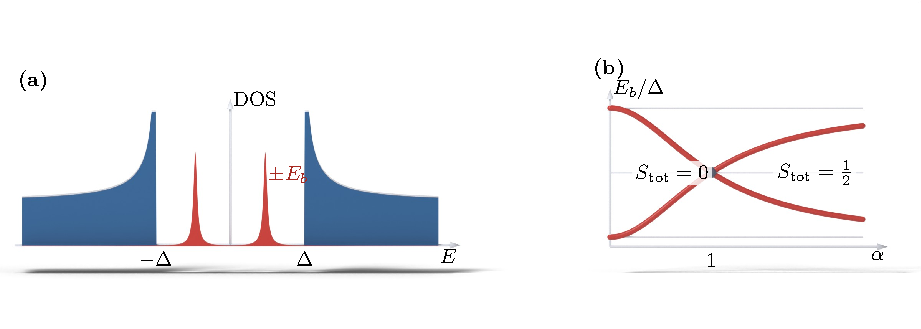
\includegraphics{figures/pdf/s09f03_ysr.pdf}
\end{aqmfigure}
